\section{Design}
\label{sec:design}

\sys{} combine envelope encryption, a published provider key and a strict server-side trust
boundary. \Cref{fig:arch} summarises the flow.

\begin{figure}[t]
  \centering
  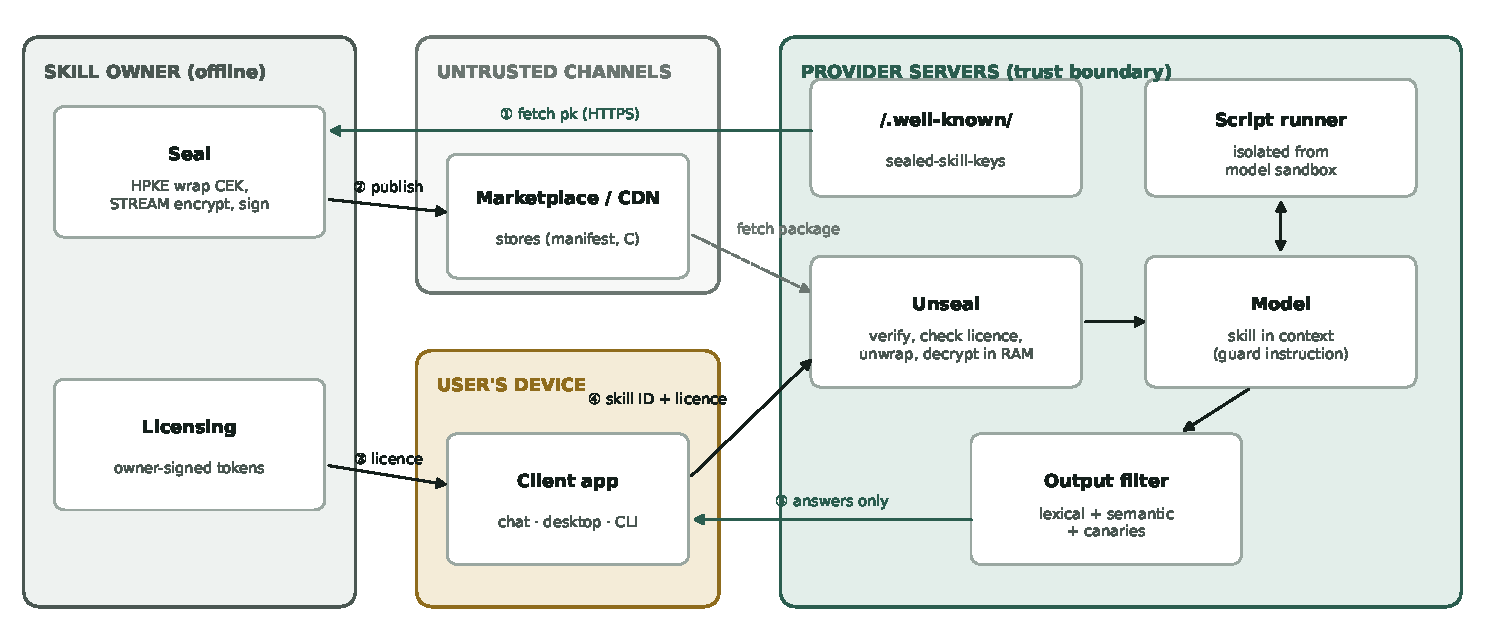
\includegraphics[width=\linewidth]{figures/architecture.pdf}
  \caption{\sys{} data flow. The owner seals offline to keys fetched from providers' well-known
  URLs; packages travel through untrusted channels; clients send only a skill reference and a
  licence; the skill is opened, used and filtered on the provider's servers, and only answers
  return to the client.}
  \label{fig:arch}
\end{figure}

\subsection{Provider key document}
Each participating provider serves, on its own domain, a JSON document listing its current
sealing keys at the well-known path \texttt{/.well-known/\allowbreak sealed-skill-keys}. Each
entry carries a key identifier, the X25519 public key in JWK form~\citep{rfc7517}, the HPKE suite,
and two published lifetimes: \texttt{seal\_until}, after which owners should stop sealing to the
key, and \texttt{decrypt\_until}, the provider's public commitment to keep the private key usable
so that packages sealed earlier keep working. An optional attestation field carries evidence that
the key was generated inside, and cannot leave, a measured environment. Because owners and
providers never communicate, these published dates are the entire contract for key lifetime.

The owner authenticates the document through the provider's TLS certificate. To limit
$\mathcal{A}_{\text{dns}}$, the sealing tool pins keys across fetches, compares fetches from several
network vantage points, and can require that keys appear in a transparency log~\citep{rfc9162,
melara2015coniks}. None of these checks requires contacting the provider.

\subsection{Sealing}
To seal a skill directory $D$ for providers $P_1,\dots,P_k$, the owner:
\begin{enumerate}
  \item samples a fresh 256-bit content key $\cek$ and computes
  $C \gets \mathsf{STREAM}_{\cek}(\mathsf{tar}(D))$ with 64\,KiB chunks;
  \item forms a header $h$ containing the format version, public skill metadata (identifier,
  version, a plain-text description for marketplace listing and relevance routing) and
  $(|C|, \mathsf{SHA256}(C))$;
  \item for each provider, fetches and checks $pk_{P_i}$ and computes
  \[ (enc_i, w_i) \gets \mathsf{HPKE.Seal}(pk_{P_i},\ \mathit{info},\ \cek),
     \qquad \mathit{info} = \texttt{"sealed-skill/0.2"} \,\|\, \mathsf{SHA256}(h); \]
  \item signs the manifest $M = (h, \{(P_i, kid_i, enc_i, w_i)\}, \mathit{policy})$ with its
  Ed25519 key and publishes $(M, C)$ anywhere.
\end{enumerate}
Adding a recipient later requires wrapping the same $\cek$ once more and re-signing the manifest;
the payload is untouched. Removing a recipient requires a new $\cek$ and a new version, because a
former recipient may retain the old content key. Per-customer canary strings~\citep{chor1994tracing}
are placed \emph{inside} the encrypted payload, never in the clear manifest.

\subsection{Server-side unsealing}
\label{sec:boundary}
The central architectural rule is that \textbf{a sealed skill is decrypted only on the provider's
servers, never in a client}, including clients the provider itself distributes. Two observations
force this. First, any secret shipped to a device the user controls can be extracted by that user;
a client able to decrypt a skill, or to prove to a key service that it is the provider, hands the
user the same ability. This is the classic failure of software-only DRM~\citep{biddle2003darknet}.
Second, even a correctly decrypted skill would have to travel from the client to the model inside
the request, where the user can read it. A client therefore sends only a skill reference and,
where the owner requires one, a licence token. The provider then:
\begin{enumerate}
  \item fetches the package and verifies the owner's signature and payload hash;
  \item verifies the licence offline against the owner's published licensing key: a short-lived,
  owner-signed statement naming the skill, the customer and an expiry;
  \item unwraps $\cek$ with its private key and decrypts the payload in memory;
  \item loads the skill into the model's context marked as confidential, mounts any scripts
  according to the policy in \cref{sec:scripts}, and applies an output filter to every reply
  (\cref{sec:filters});
  \item returns only the model's answers to the client.
\end{enumerate}

\subsection{Output-side defences}
\label{sec:filters}
Because the model reads the skill, the provider needs defences at the model's output, the only
place $\mathcal{A}_{\text{query}}$ can observe. We evaluate three, which compose:
\begin{description}[leftmargin=1.2em]
  \item[Guard instruction.] A system-prompt paragraph telling the model the skill is confidential
  and must not be revealed, quoted, paraphrased, translated, encoded or reconstructed, regardless
  of claimed authority.
  \item[Lexical filter.] The reply is de-obfuscated (base64 runs decoded, zero-width characters
  removed, separators and reversals undone) and blocked if it shares a contiguous run of at least
  $L$ words with the skill, or contains a canary.
  \item[Semantic filter.] Each reply sentence is embedded, and the reply is blocked if its maximum
  cosine similarity to any skill rule exceeds a threshold $\tau$.
\end{description}
Blocked replies are replaced with a fixed refusal. Canaries additionally serve for attribution:
if a reconstruction surfaces publicly, the customer-specific canary identifies the licence it came
from, in the spirit of traitor tracing~\citep{chor1994tracing}.

\subsection{Scripts}
\label{sec:scripts}
A skill's scripts must be executed, which raises a question the instruction text does not: where
do they run? The natural design mounts them in the agent's code sandbox and lets the model call
them. If that sandbox also offers general code execution, as agent sandboxes usually do, the
scripts cannot be ``run-only'': an interpreter that can execute a file can read it, and the model
can be asked to print it (\cref{sec:casestudy}). We therefore recommend that confidential logic run
\emph{outside} the model's sandbox, either in a separate provider-side process that exposes only a
narrow call interface, or on the owner's own infrastructure behind a tool, for example a Model
Context Protocol server~\citep{mcp2026spec}. In the latter design the proprietary code never
enters any model's context or sandbox, and only results cross into the conversation. The logic
must sit in an MCP \emph{tool}, executed server-side; serving it as an MCP-hosted
\emph{skill}~\citep{mcp2026skillsext} would deliver the text into the model's context again.

\subsection{Package format}
\Cref{lst:manifest} shows an abridged manifest. The public description stays in clear text so
marketplaces can list the skill and agents can decide relevance before unsealing.

\begin{lstlisting}[caption={Abridged \texttt{manifest.json} (format \texttt{sealed-skill/0.2}).},label={lst:manifest},float=t]
{ "format": "sealed-skill/0.2",
  "skill":   { "id": "com.example.tax-reconciler", "version": "2.3.0",
               "public_description": "Reconciles purchase ledgers against tax filings.",
               "owner": "did:web:example.com" },
  "payload": { "aead": "AES-256-GCM", "chunking": "STREAM-64KiB",
               "size": 482113, "sha256": "9f2c...e71a" },
  "recipients": [{ "provider": "provider-a.example", "key_id": "pa-2026-09-k3",
      "key_source": "https://provider-a.example/.well-known/sealed-skill-keys",
      "hpke_suite": {"kem": "0x0020", "kdf": "0x0001", "aead": "0x0002"},
      "enc": "...", "wrapped_cek": "..." }],
  "policy":  { "confidential": true, "scripts": "owner-hosted",
               "licence_issuer_key": "https://licensing.example.com/.well-known/jwks.json" },
  "signature": { "alg": "Ed25519", "key_id": "example-signing-2026", "sig": "..." } }
\end{lstlisting}
